\section*{第四章 参数方程、极坐标}

\section*{一、参数方程}

\section*{【典型题型和解题技巧】}

1. 消参的技巧.

主要的消参方法有:

(1)代入法.

例 1 将参数方程 $\left\{  \begin{array}{l} x = \dfrac{3{t}^{2}}{1 + {t}^{2}}, \\  y = \dfrac{5 - {t}^{2}}{1 + {t}^{2}} \end{array}\right.$ ( $t$ 为参数)化为普通方程.

解 由第一式 $x + {t}^{2}x = 3{t}^{2}$ ,即 $\left( {3 - x}\right) {t}^{2} = x$ ,显然 $x \neq  3,\therefore {t}^{2} = \dfrac{x}{3 - x}$ ,

代入第二式, $y = \dfrac{5 - \dfrac{x}{3 - x}}{1 + \dfrac{x}{3 - x}} = \dfrac{{15} - {6x}}{3} = 5 - {2x}$ ,即 ${2x} + y - 5 = 0$ . 又 ${t}^{2} = \dfrac{x}{3 - x} \geq  0$ .

$\therefore 0 \leq  x < 3$ . 故所求普通方程为 ${2x} + y - 5 = 0\left( {0 \leq  x < 3}\right)$ .

注意 将参数方程化为普通方程时,不能任意缩小或扩大曲线中 $x$ , $y$ 的取值范围.

(2)加减法.

例 2 若 $\left\{  {\begin{array}{l} x = {a}^{t} + {a}^{-t}, \\  y = {a}^{t} - {a}^{-t} \end{array}\left( {a > 0,a \neq  1,t\text{ 为参数 }}\right) }\right.$ ,求点(x, y)轨迹的普通方程.

解 两式平方相减 ${x}^{2} - {y}^{2} = {\left( {a}^{t} + {a}^{-t}\right) }^{2} - {\left( {a}^{t} - {a}^{-t}\right) }^{2} = 4$ ,而 ${a}^{t} + {a}^{-t} \geq  2$ .

故所求轨迹的方程为 ${x}^{2} - {y}^{2} = 4\left( {x \geq  2}\right)$ .

(3) 换元法.

例 3 将参数方程 $\left\{  \begin{array}{l} x = \dfrac{t}{1 + {t}^{2}}, \\  y = \dfrac{1 - {t}^{2}}{1 + {t}^{2}} \end{array}\right.$ ( $t$ 为参数)化为普通方程.

解 令 $t = \tan \dfrac{\theta }{2}$ ,则 $\left\{  {\begin{array}{l} x = \dfrac{1}{2}\sin \theta , \\  y = \cos \theta , \end{array}\therefore 4{x}^{2} + {y}^{2} = 1}\right.$ .

又 $y = \dfrac{1 - {t}^{2}}{1 + {t}^{2}}$ ,显然 $y \neq   - 1$ . $\therefore$ 所求的普通方程为 $4{x}^{2} + {y}^{2} = 1\left( {y \neq   - 1}\right)$ . 2. 直线参数方程的应用. 过定点 $\left( {{x}_{0},{y}_{0}}\right)$ ,倾角为 $\alpha$ 的直线参数方程为 $\left\{  \begin{array}{l} x = {x}_{0} + t\cos \alpha , \\  y = {y}_{0} + t\sin \alpha  \end{array}\right.$ ( $t$ 为参数). 参数 $t$ 的几何意义是:

(1) $\left| t\right|$ 表示直线上的点(x, y)和定点 $\left( {{x}_{0},{y}_{0}}\right)$ 的距离；

(2)当点(x, y)在点 $\left( {{x}_{0},{y}_{0}}\right)$ 的上方时, $t > 0$ ；

当点(x, y)在点 $\left( {{x}_{0},{y}_{0}}\right)$ 的下方时, $t < 0$ ;

当点(x, y)与点 $\left( {{x}_{0},{y}_{0}}\right)$ 重合时, $t = 0$ .

反之亦然.

方程 (*) 的主要应用有:

(1) 求一端是 $P\left( {{x}_{0},{y}_{0}}\right)$ 的线段长.

例 4 直线 ${l}_{1}$ 过点 $P\left( {4,3}\right)$ ,且倾斜角为 $\arctan \dfrac{2}{3}$ .

(1) 求 ${l}_{1}$ 的参数方程.

(2)若 ${l}_{1}$ 和直线 ${l}_{2} : x + y - 2 = 0$ 交于点 $Q$ ,求 $\left| {PQ}\right|$ .

解 (1) ${l}_{1}$ 的倾斜角 $\alpha$ 满足 $\tan \alpha  = \dfrac{2}{3}$ ,

$\therefore \sin \alpha  = \dfrac{2\sqrt{13}}{13},\cos \alpha  = \dfrac{3\sqrt{13}}{13}$ .

${l}_{1}$ 的参数方程为 $\left\{  {\begin{array}{l} x = 4 + \dfrac{3\sqrt{13}}{13}t, \\  y = 3 + \dfrac{2\sqrt{13}}{13}t \end{array}\text{ ( }t}\right.$ 为参数).

(2)将上述方程代入 $x + y - 2 = 0$ ,得 $4 + \dfrac{3}{\sqrt{13}}t + 3 + \dfrac{2}{\sqrt{13}}t - 2 = 0$ ,得 $t =  - \sqrt{13}$ , $\therefore \left| {PQ}\right|  = \left| t\right|  = \sqrt{13}$ . (2)求弦长.

例 5 如图 1,过点 $P\left( {2,2}\right)$ ,倾斜角为 $\arccos \left( {-\dfrac{\sqrt{3}}{3}}\right)$ 的直线与曲线 $5{x}^{2} - 4{y}^{2} + {10x} + {16y} - {31} = 0$ 交于 $A,B$ 两点,求 $\left| {AB}\right|$ .

\begin{center}
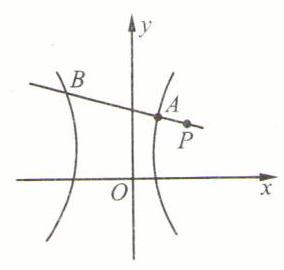
\includegraphics[width=0.2\textwidth]{bodyxb/src/bo_d20aucref24c73anc48g_108_1173_1686_284_270_0.jpg}
\end{center}


(图 1)

解 直线的参数方程为 $\left\{  \begin{array}{l} x = 2 - \dfrac{\sqrt{3}}{3}t, \\  y = 2 + \dfrac{\sqrt{6}}{3}t. \end{array}\right.$

代入双曲线方程并化简得 ${t}^{2} + {10}\sqrt{3}t - {25} = 0$ ,

则 $\left| {{t}_{1} - {t}_{2}}\right|  - \sqrt{{\left( {t}_{1} - {t}_{2}\right) }^{2}} - \sqrt{{\left( {t}_{1} + {t}_{2}\right) }^{2} - 4{t}_{1}{t}_{2}} = \sqrt{{300} + {100}} = {20}$ .

$\therefore \left| {AB}\right|  = \left| {{t}_{1} - {t}_{2}}\right|  = {20}$ .

注意 利用直线的参数方程(*)求二次曲线的弦长时,可将 (*) 式代入二次曲线方程得: $a{t}^{2} + {bt} + c = 0$ . 弦长为 $\left| {{t}_{1} - {t}_{2}}\right|  = \sqrt{{\left( {t}_{1} - {t}_{2}\right) }^{2}} = \sqrt{{\left( {t}_{1} + {t}_{2}\right) }^{2} - 4{t}_{1}{t}_{2}} = \sqrt{{\left( -\dfrac{b}{a}\right) }^{2} - \dfrac{4c}{a}}$ .

( 3 )求线段长度之积 $\left| {PA}\right|  \cdot  \left| {PB}\right|$ .

例 6 过点 $P\left( {1, - 2}\right)$ ,且倾斜角为 ${45}^{ \circ  }$ 的直线 $l$ 与椭圆 ${x}^{2} + 2{y}^{2} = 8$ 交于两点 $A,B$ (如图 2 ),求 $\left| {PA}\right|  \cdot  \left| {PB}\right|$ .

解 $l$ 的参数方程为 $\left\{  \begin{array}{l} x = 1 + \dfrac{1}{\sqrt{2}}t, \\  y =  - 2 + \dfrac{1}{\sqrt{2}}t. \end{array}\right.$

\begin{center}
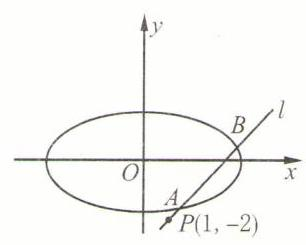
\includegraphics[width=0.2\textwidth]{bodyxb/src/bo_d20aucref24c73anc48g_109_1147_529_306_245_0.jpg}
\end{center}


(图 2)

代入 ${x}^{2} + 2{y}^{2} - 8 = 0$ ,并化简得 $\dfrac{3}{2}{t}^{2} - 3\sqrt{2}t + 1 = 0$ ,

于是 $\left| {PA}\right|  \cdot  \left| {PB}\right|  = \left| {{t}_{1} \cdot  {t}_{2}}\right|  = \dfrac{2}{3}$ .

3. 圆锥曲线参数方程的应用.

例 7 设直线 ${Ax} + {By} + C = 0$ 和半圆 $y = \sqrt{1 - {x}^{2}}$ 交于 $M,N$ 两点, ${OM},{ON}$ 的倾斜角分别为 $\alpha ,\beta \left( {\alpha  + \beta  \neq  \pi }\right) ,O$ 为原点,求 $\sin \left( {\alpha  + \beta }\right)$ .

解 如图 3,半圆方程即 ${x}^{2} + {y}^{2} = 1\left( {y \geq  0}\right)$ .

可设点 $M,N$ 的坐标分别为 $\left( {\cos \alpha ,\sin \alpha }\right) ,\left( {\cos \beta ,\sin \beta }\right)$ ,

则 $\left\{  \begin{array}{l} A\cos \alpha  + B\sin \alpha  + C = 0, \\  A\cos \beta  + B\sin \beta  + C = 0. \end{array}\right.$

\begin{center}
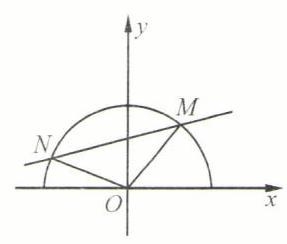
\includegraphics[width=0.2\textwidth]{bodyxb/src/bo_d20aucref24c73anc48g_109_1162_1241_287_244_0.jpg}
\end{center}


(图 3)

两式相减并和差化积,得 $- 2\sin \dfrac{\alpha  - \beta }{2}\left( {A\sin \dfrac{\alpha  + \beta }{2} - B\cos \dfrac{\alpha  + \beta }{2}}\right)  = 0$ .

由题设, $\sin \dfrac{\alpha  - \beta }{2} \neq  0,A \neq  0$ ,于是 $\tan \dfrac{\alpha  + \beta }{2} = \dfrac{B}{A}$ ,

$\therefore \sin \left( {\alpha  + \beta }\right)  = \dfrac{2AB}{{A}^{2} + {B}^{2}}.$

例 8 点 $P$ 在圆 ${O}^{\prime } : {x}^{2} + {\left( y - 2\right) }^{2} = \dfrac{1}{4}$ 上移动,点 $Q$ 在椭圆 ${x}^{2} + 4{y}^{2} = 4$ 上移动 (图 4),求 $\left| {PQ}\right|$ 的最大值及相应的点 $Q$ 的坐标.

解 $\left| {PQ}\right|  \leq  \left| {P{O}^{\prime }}\right|  + \left| {{O}^{\prime }Q}\right|  = \dfrac{1}{2} + \left| {{O}^{\prime }Q}\right|$ .

\begin{center}
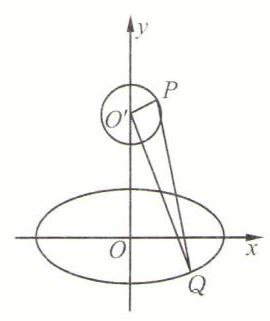
\includegraphics[width=0.2\textwidth]{bodyxb/src/bo_d20aucref24c73anc48g_109_1180_1809_270_321_0.jpg}
\end{center}


(图 4)

设点 $Q$ 的坐标为 $\left( {2\cos \alpha ,\sin \alpha }\right)$ ,而 ${O}^{\prime }\left( {0,2}\right)$ ,则

${\left| {O}^{\prime }Q\right| }^{2} = 4{\cos }^{2}\alpha  + {\left( \sin \alpha  - 2\right) }^{2} =  - 3{\left( \sin \alpha  + \dfrac{2}{3}\right) }^{2} + \dfrac{28}{3} \leq  \dfrac{28}{3}.$

$\therefore \left| {{O}^{\prime }Q}\right|  \leq  \dfrac{2}{3}\sqrt{21}$ ,此时 $\sin \alpha  =  - \dfrac{2}{3},\cos \alpha  =  \pm  \dfrac{\sqrt{5}}{3}$ .

$\therefore \left| {PQ}\right|$ 的最大值是 $\dfrac{1}{2} + \dfrac{2}{3}\sqrt{21}$ ,相应的点 $Q$ 的坐标为 $\left( {\pm \dfrac{2}{3}\sqrt{5}, - \dfrac{2}{3}}\right)$ .

注意 二次曲线常用的参数方程由如下形式给出:

${\left( x - {x}_{0}\right) }^{2} + {\left( y - {y}_{0}\right) }^{2} = {R}^{2},\left\{  {\begin{array}{l} x = {x}_{0} + R\cos \alpha , \\  y = {x}_{0} + R\sin \alpha  \end{array}\text{ ( }\alpha }\right.$ 为参数).

$\dfrac{{\left( x - {x}_{0}\right) }^{2}}{{a}^{2}} + \dfrac{{\left( y - {y}_{0}\right) }^{2}}{{b}^{2}} = 1,\left\{  {\begin{array}{l} x = {x}_{0} + a\cos \alpha , \\  y = {y}_{0} + b\sin \alpha  \end{array}\text{ (α 为参数). }}\right.$

$\dfrac{{\left( x - {x}_{0}\right) }^{2}}{{a}^{2}} - \dfrac{{\left( y - {y}_{0}\right) }^{2}}{{b}^{2}} = 1,\left\{  \begin{array}{l} x = {x}_{0} + \dfrac{a}{\cos \alpha }, \\  y = {y}_{0} + b\tan \alpha  \end{array}\right.$ ( $\alpha$ 为参数).

${\left( y - {y}_{0}\right) }^{2} = {2p}\left( {x - {x}_{0}}\right) ,\left\{  {\begin{array}{l} x = {x}_{0} + {2p}{t}^{2}, \\  y = {y}_{0} + {2pt} \end{array}\text{ ( }t}\right.$ 为参数). 4. 参数法求轨迹.

(1) $k$ 参数.

例 9 过抛物线 ${y}^{2} = {2px}\left( {p > 0}\right)$ 的顶点作两条互相垂直的弦 ${OA},{OB}$ (图 5).

(1)设 ${OA}$ 的斜率为 $k$ ,试用 $k$ 表示点 $A,B$ 的坐标.

\begin{center}
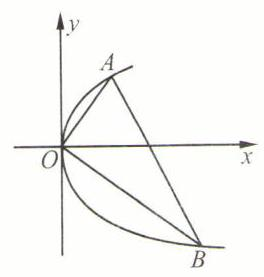
\includegraphics[width=0.2\textwidth]{bodyxb/src/bo_d20aucref24c73anc48g_110_1197_980_264_277_0.jpg}
\end{center}


(图 5)

(2)求弦 ${AB}$ 的中点 $M$ 的轨迹方程.

解 (1) 解方程组 $\left\{  \begin{array}{l} y = {kx}, \\  {y}^{2} = {2px}, \end{array}\right.$ 得 ${x}_{A} = \dfrac{2p}{{k}^{2}},{y}_{A} = \dfrac{2p}{k}$ .

以 $- \dfrac{1}{k}$ 替换上式中的 $k$ ,得 ${x}_{B} = {2p}{k}^{2},{y}_{B} =  - {2pk}$ .

$\therefore$ 点 $A,B$ 的坐标分别为 $A\left( {\dfrac{2p}{{k}^{2}},\dfrac{2p}{k}}\right) ,B\left( {{2p}{k}^{2}, - {2pk}}\right)$ .

(2)设弦 ${AB}$ 的中点 $M\left( {x,y}\right)$ ,则 $\left\{  \begin{array}{l} x = p\left( {{k}^{2} + \dfrac{1}{{k}^{2}}}\right) , \\  y = p\left( {\dfrac{1}{k} - k}\right) . \end{array}\right.$

消去参数 $k$ 得 ${y}^{2} = {px} - 2{p}^{2}$ ,即为点 $M$ 的轨迹方程. (2)点参数. 例 10 给出两定点 $P\left( {-2,2}\right) ,Q\left( {0,2}\right)$ ,长为 $\sqrt{2}$ 的线段 ${AB}$ 在直线 $y = x$ 上移动 (图 6),其中点 $B$ 在点 $A$ 的上方.

(1)设点 $A$ 的坐标为 $A\left( {t,t}\right)$ ,写出点 $B$ 的坐标.

\begin{center}
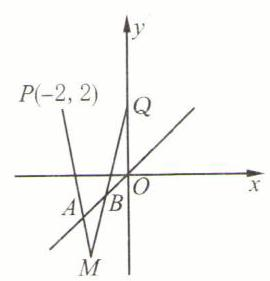
\includegraphics[width=0.2\textwidth]{bodyxb/src/bo_d20aucref24c73anc48g_110_1197_1838_270_281_0.jpg}
\end{center}


(图 6)

(2)求直线 ${PA}$ , ${QB}$ 的交点 $M$ 的轨迹方程.

解(1) $B\left( {t + 1,t + 1}\right)$ .

(2) ${l}_{PA} : \left( {t - 2}\right) \left( {x + 2}\right)  = \left( {t + 2}\right) \left( {y - 2}\right)$ .

即 $\left( {x - y + 4}\right) t = 2\left( {x + y}\right)$ ,

${l}_{QB}$ : 即 $\left( {t - 1}\right) x - \left( {t + 1}\right) \left( {y - 2}\right)$ ,

$x + y - 2 = \left( {x - y + 2}\right) t.$

两式相乘,消去参数 $t$ ,并化简得 ${\left( y + 1\right) }^{2} - {\left( x + 1\right) }^{2} = 8$ ,此即为交点 $M$ 的轨迹方程.

(3) $\lambda$ 参数.

例 11 如图 7,过点 $P\left( {4,1}\right)$ 作直线和椭圆 $\dfrac{{x}^{2}}{3} + \dfrac{{y}^{2}}{4} = 1$ 交于点 $A\left( {{x}_{1},{y}_{1}}\right) ,B\left( {{x}_{2},{y}_{2}}\right) \left( {{x}_{1} > }\right.$  $\left. {x}_{2}\right) ,Q$ 是线段 ${AB}$ 上的点, $\vv{AP} = \lambda \vv{PB},\vv{AQ} =  - \lambda \vv{QB}$ ,求点 $Q$ 的轨迹方程.

解 设点 $Q$ 的坐标为(x, y),由 $\vv{AP} = \lambda \vv{PB}$ 和 $\vv{AQ} =  - \lambda \vv{QB}$ ,得 $4 =$  $\dfrac{{x}_{1} + \lambda {x}_{2}}{1 + \lambda },1 = \dfrac{{y}_{1} + \lambda {y}_{2}}{1 + \lambda },x = \dfrac{{x}_{1} - \lambda {x}_{2}}{1 - \lambda },y = \dfrac{{y}_{1} - \lambda {y}_{2}}{1 - \lambda }.$

\begin{center}
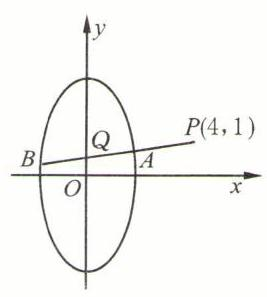
\includegraphics[width=0.2\textwidth]{bodyxb/src/bo_d20aucref24c73anc48g_111_1179_477_267_297_0.jpg}
\end{center}


(图 7)

$\therefore {4x} = \dfrac{{x}_{1}^{2} - {\lambda }^{2}{x}_{2}^{2}}{1 - {\lambda }^{2}},y = \dfrac{{y}_{1}^{2} - {\lambda }^{2}{y}_{2}^{2}}{1 - {\lambda }^{2}}$ ,

即 ${16x} = \dfrac{4{x}_{1}^{2} - 4{\lambda }^{2}{x}_{2}^{2}}{1 - {\lambda }^{2}},{3y} = \dfrac{3{y}_{1}^{2} - 3{\lambda }^{2}{y}_{2}^{2}}{1 - {\lambda }^{2}}$ .

两式相加,得

${16x} + {3y} = \dfrac{\left( {4{x}_{1}^{2} + 3{y}_{1}^{2}}\right)  - {\lambda }^{2}\left( {4{x}_{2}^{2} + 3{y}_{2}^{2}}\right) }{1 - {\lambda }^{2}} = {12} \cdot  \dfrac{1 - {\lambda }^{2}}{1 - {\lambda }^{2}} = {12}.$

$\therefore$ 点 $Q$ 的轨迹方程为 ${16x} + {3y} - {12} = 0$ (在已知椭圆的内部).

(4)角参数.

例 12 如图 8,边长为 $a$ 的等边三角形 ${ABC}$ 的两个端点 $A,B$ 分别在 $x$ 轴正半轴、 $y$ 轴正半轴上移动,顶点 $C$ 和原点 $O$ 分别在 ${AB}$ 两侧,记 $\angle {CAx} = \alpha$ ,求顶点 $C$ 的轨迹的参数方程.

\begin{center}
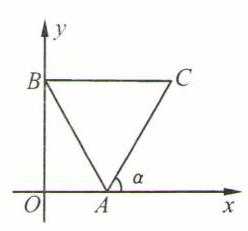
\includegraphics[width=0.2\textwidth]{bodyxb/src/bo_d20aucref24c73anc48g_111_1197_1104_248_231_0.jpg}
\end{center}


(图 8)

解 过点 $C$ 作 ${CD} \bot  x$ 轴于点 $D$ ,设 $C\left( {x,y}\right)$ ,

由 $\left\{  \begin{array}{l} x = {OA} + {AD}, \\  y = {DC}, \end{array}\right.$ 得 $\left\{  \begin{array}{l} x = a\cos \left( {{120}^{ \circ  } - \alpha }\right)  + a\cos \alpha , \\  y = a\sin \alpha , \end{array}\right.$

即为顶点 $C$ 的轨迹的参数方程.

\section*{【训练题】}

(A)

1. 与普通方程 ${xy} = 1$ 表示相同曲线的参数方程 ( $t$ 为参数) 是 (   )

(A) $\left\{  \begin{array}{l} x = {t}^{2}, \\  y = {t}^{-2}. \end{array}\right.$ (B) $\left\{  \begin{array}{l} x = \sin t, \\  y = \dfrac{1}{\sin t}. \end{array}\right.$ (C) $\left\{  \begin{array}{l} x = \cos t, \\  y = \dfrac{1}{\cos t}. \end{array}\right.$ (D) $\left\{  \begin{array}{l} x = \tan t, \\  y = \cot t. \end{array}\right.$

2. 若曲线 $\left\{  \begin{array}{l} x = 1 + \cos {2\theta }, \\  y = {\sin }^{2}\theta  \end{array}\right.$ ( $\theta$ 为参数),则点(x, y)的轨迹是 (   )

(A) 直线 $x + {2y} - 2 = 0$ . (B) 以(2,0)为端点的射线.

(C) 圆 ${\left( x - 1\right) }^{2} + {y}^{2} = 1$ . (D) 以(2,0)和(0,1)为端点的线段.

3. 曲线 $\left\{  \begin{array}{l} x = t - 8, \\  y = {t}^{2} - t \end{array}\right.$ ( $t$ 为参数)与 $x$ 轴的交点坐标是 (   )

(A) $\left( {8,0}\right) ,\left( {-7,0}\right)$ . (B) $\left( {-8,0}\right) ,\left( {-7,0}\right)$ .

(C) $\left( {8,0}\right) ,\left( {7,0}\right)$ . (D) $\left( {-8,0}\right) ,\left( {7,0}\right)$ .

4. 参数方程 $\left\{  \begin{array}{l} x = \sin \theta  + \cos \theta , \\  y = \sin \theta  \cdot  \cos \theta  \end{array}\right.$ ( $\theta$ 为参数)表示的曲线为(   )

\begin{center}
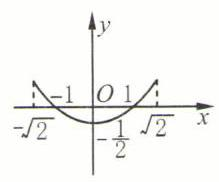
\includegraphics[width=0.2\textwidth]{bodyxb/src/bo_d20aucref24c73anc48g_112_312_494_219_182_0.jpg}
\end{center}


(A)

\begin{center}
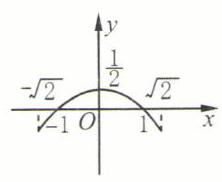
\includegraphics[width=0.2\textwidth]{bodyxb/src/bo_d20aucref24c73anc48g_112_572_492_222_182_0.jpg}
\end{center}


(B)

\begin{center}
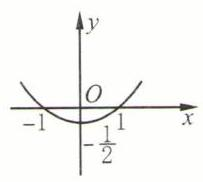
\includegraphics[width=0.2\textwidth]{bodyxb/src/bo_d20aucref24c73anc48g_112_837_491_203_182_0.jpg}
\end{center}


(C)

\begin{center}
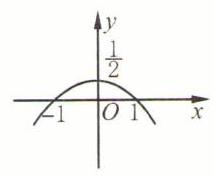
\includegraphics[width=0.2\textwidth]{bodyxb/src/bo_d20aucref24c73anc48g_112_1078_491_213_176_0.jpg}
\end{center}


(D)

5. 由方程 ${x}^{2} + {y}^{2} - {4tx} - {2ty} + 3{t}^{2} - 4 = 0$ ( $t$ 为参数) 所表示的一族圆的圆心轨迹是 (   )

(A) 一个定点. (B) 一个椭圆.

(C) 一条抛物线. (D) 一条直线.

6. 参数方程 $\left\{  \begin{array}{l} x = {\cos }^{2}\theta , \\  y = \sin \theta  \end{array}\right.$ ( $\theta$ 为参数)所表示的曲线是 (   )

\begin{center}
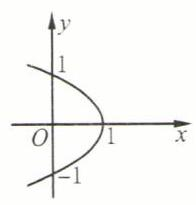
\includegraphics[width=0.2\textwidth]{bodyxb/src/bo_d20aucref24c73anc48g_112_319_1037_196_205_0.jpg}
\end{center}


(A)

\begin{center}
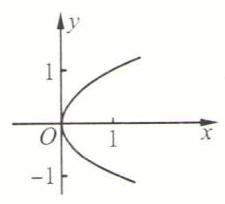
\includegraphics[width=0.2\textwidth]{bodyxb/src/bo_d20aucref24c73anc48g_112_570_1037_225_204_0.jpg}
\end{center}


(B)

\begin{center}
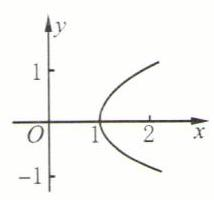
\includegraphics[width=0.2\textwidth]{bodyxb/src/bo_d20aucref24c73anc48g_112_847_1035_214_200_0.jpg}
\end{center}


(C)

\begin{center}
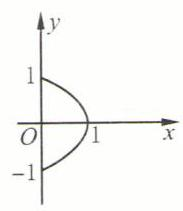
\includegraphics[width=0.2\textwidth]{bodyxb/src/bo_d20aucref24c73anc48g_112_1110_1028_183_211_0.jpg}
\end{center}


(D)

7. 直线 $\left\{  \begin{array}{l} x =  - 2 + t\cos {30}^{ \circ  }, \\  y = 3 - t\sin {60}^{ \circ  } \end{array}\right.$ ( $t$ 为参数)的倾斜角 $\alpha$ 等于(   )

(A) ${30}^{ \circ  }$ . (B) ${60}^{ \circ  }$ . (C) $- {45}^{ \circ  }$ . (D) ${135}^{ \circ  }$ .

8. 过点(5, - 4),倾斜角为 $\pi  - \arctan \dfrac{4}{5}$ 的直线 $l$ 的参数方程是(   )

(A) $\left\{  \begin{array}{l} x = 5 + {5t}, \\  y =  - 4 - {9t} \end{array}\right.$ ( $t$ 为参数). (B) $\left\{  {\begin{array}{l} x = 5 - {5t}, \\  y =  - 4 + {4t} \end{array}\text{ ( }t}\right.$ 为参数).

(C) $\left\{  {\begin{array}{l} x = 5 + {5t}, \\  y =  - 4 + {4t} \end{array}\text{ ( }t}\right.$ 为参数). (D) $\left\{  {\begin{array}{l} x = 5 - {5t}, \\  y =  - 4 - {4t} \end{array}\text{ ( }t}\right.$ 为参数).

9. 将下列参数方程化为普通方程 ( $t$ 为参数).

(1) $\left\{  \begin{array}{l} x = \sin t, \\  y = 1 + \cos {2t} \end{array}\right.$ :\blkda{}. (2) $\left\{  \begin{array}{l} x = 1 + {\cos }^{2}t, \\  y = {\sin }^{2}t - {\sin }^{4}t \end{array}\right.$ :\blkda{}.

(3) $\left\{  \begin{array}{l} x = \dfrac{2 - {3t}}{1 + t}, \\  y = \dfrac{1 + {4t}}{1 + t} \end{array}\right.$ :\blkda{}. (4) $\left\{  \begin{array}{l} x = t + \dfrac{1}{t}, \\  y = {t}^{2} + \dfrac{1}{{t}^{2}}, \end{array}\right.$ :\blkda{}.

*10. (1) 直线 $\left\{  \begin{array}{l} x = 3 + {at}, \\  y =  - 1 + {bt} \end{array}\right.$ ( $t$ 为参数) 过定点\blkda{}. 若 ${ab} > 0$ ,则它的倾斜角为\blkda{}; 若 ${ab} < 0$ ,则它的倾斜角为\blkda{}.

(2)若直线 $\left\{  \begin{array}{l} x = 4 + {at}, \\  y = {bt} \end{array}\right.$ ( $t$ 为参数)与曲线 ${x}^{2} + {y}^{2} - {4x} + 1 = 0$ 相切,则这条直线的倾斜角等于\blkda{}.

(3) 过点 $P\left( {4,3}\right)$ 的直线 ${l}_{1}$ 的参数方程为 $\left\{  \begin{array}{l} x = 4 + \dfrac{6\sqrt{13}}{13}t, \\  y = 3 + \dfrac{4\sqrt{13}}{13}t, \end{array}\right.$ 它与直线 ${l}_{2} : x + y - 2 = 0$ 的交点为 $Q$ ,则 $\left| {PQ}\right|  =$ \blkda{}.

(4) 过点 $P\left( {4, - 1}\right)$ 且与直线 $l : \left\{  \begin{array}{l} x = 3 + \dfrac{4}{5}t, \\  y =  - 2 + \dfrac{3}{5}t \end{array}\right.$ ( $t$ 为参数) 平行的直线在 $y$ 轴上的截距是\blkda{}.

(5)若直线 $\left\{  \begin{array}{l} x = 1 - {3t}, \\  y = 2 + {4t} \end{array}\right.$ ( $t$ 为参数)上的点 $P$ 到点(1,2)的距离为 2,则点 $P$ 的坐标为\blkda{}.

*11. (1) 椭圆 $\left\{  \begin{array}{l} x = 4 + 2\cos \varphi , \\  y = 1 + 5\sin \varphi  \end{array}\right.$ ( $\varphi$ 为参数)的焦距等于\blkda{}.

(2)双曲线 $\left\{  \begin{array}{l} x = 1 + \sqrt{3}\tan \theta , \\  y =  - 2 + \dfrac{3}{\cos \theta } \end{array}\right.$ ( $\theta$ 为参数)的两条渐近线的夹角为\blkda{}.

(3)椭圆 $\left\{  \begin{array}{l} x = 4\cos \theta  + 1, \\  y = 3\sin \theta  \end{array}\right.$ ( $\theta$ 为参数)的左焦点坐标是\blkda{}.

(4)抛物线 $\left\{  \begin{array}{l} x = {2t}, \\  y = 2{t}^{2} + 1 \end{array}\right.$ ( $t$ 为参数)的准线的普通方程是\blkda{}.

12. (1) 已知过点 $A\left( {2,0}\right)$ 的直线与抛物线 $y = {x}^{2}$ 交于不同的两点 $E,F$ ,求线段 ${EF}$ 中点 $P$ 的轨迹方程.

(2)若关于 $x$ 的二次方程 ${x}^{2} - {ax} + b = 0$ 的两个根为直角三角形的两锐角的正弦,求点 (a, b)的轨迹的普通方程.

(3)已知抛物线 $y = \dfrac{1}{4}{x}^{2}$ 与直线 ${tx} - {2y} + {2t} = 0$ ( $t$ 为参数)相交,求此直线被抛物线截得的线段中点的轨迹方程.

\section*{(B)}

* 13. 直线 $\left\{  {\begin{array}{l} x = 1 + {2t}, \\  y = 2 + t \end{array}\text{ ( }t}\right.$ 为参数) 被圆 ${x}^{2} + {y}^{2} = 9$ 截得的弦长等于(   )

(A) $\dfrac{12}{5}$ . (B) $\dfrac{{12}\sqrt{5}}{5}$ . (C) $\dfrac{9\sqrt{2}}{5}$ . (D) $\dfrac{9\sqrt{10}}{5}$ .

14. 若曲线 $\left\{  \begin{array}{l} x = {2pt}, \\  y = {2p}{t}^{2} \end{array}\right.$ ( $t$ 为参数)上异于原点的不同两点 ${M}_{1},{M}_{2}$ 所对应的参数分别是 ${t}_{1},{t}_{2}$ , 则弦 ${M}_{1}{M}_{2}$ 所在直线的斜率是 (   )

(A) ${t}_{1} + {t}_{2}$ . (B) ${t}_{1} - {t}_{2}$ . (C) $\dfrac{1}{{t}_{1} + {t}_{2}}$ . (D) $\dfrac{1}{{t}_{1} - {t}_{2}}$ .

*15. 直线 $\left\{  \begin{array}{l} x =  - 2 - \sqrt{2}t, \\  y = 3 + \sqrt{2}t \end{array}\right.$ ( $t$ 为参数)上与点 $P\left( {-2,3}\right)$ 的距离等于 $\sqrt{2}$ 的点的坐标是 (   )

(A)(-4,5). (B)(-3,4).

(C)(-3,4)或(-1,2). (D)(-4,5)或(0,1).

*16. 直线 $\left\{  \begin{array}{l} x = 2 + t, \\  y = \sqrt{3}t \end{array}\right.$ ( $t$ 为参数) 被双曲线 ${x}^{2} - {y}^{2} = 1$ 所截得的弦长是 ( )

(A) $2\sqrt{10}$ . (B) $\sqrt{10}$ . (C) $\dfrac{1}{2}\sqrt{10}$ . (D) $\dfrac{1}{3}\sqrt{10}$ .

17. 复平面上,满足 $\left| {z - \sqrt{2}{ai}}\right|  - \left| {z + \sqrt{2}{ai}}\right|  = {2a}\left( {a > 0}\right)$ 的复数 $z = x + {yi}\left( {x,y \in  \mathbf{R}}\right)$ 对应点的轨迹的参数方程是 (   )

(A) $\left\{  {\begin{array}{l} x = a\tan \theta , \\  y = \dfrac{a}{\cos \theta } \end{array}\left( {0 < \theta  < \dfrac{\pi }{2}\text{ 或 }\dfrac{\pi }{2} < \theta  < \pi }\right) .}\right.$

(B) $\left\{  {\begin{array}{l} x = a\tan \theta , \\  y = \dfrac{a}{\cos \theta } \end{array}\left( {-\dfrac{\pi }{2} < \theta  < \dfrac{\pi }{2}}\right) .}\right.$

(C) $\left\{  {\begin{array}{l} x = a\tan \theta , \\  y = \dfrac{a}{\cos \theta } \end{array}\left( {\dfrac{\pi }{2} < \theta  < \dfrac{3\pi }{2}}\right) .}\right.$

(D) $\left\{  {\begin{array}{l} x = a\tan \theta , \\  y = \dfrac{a}{\cos \theta } \end{array}\left( {\dfrac{\pi }{2} < \theta  < \dfrac{3\pi }{2}\text{ 或 }\dfrac{3\pi }{2} < \theta  < {2\pi }}\right) .}\right.$

18. 将下列参数方程化为普通方程 $(t,\theta$ 为参数):

(1) $\left\{  \begin{array}{l} x = {\mathrm{e}}^{t} + {\mathrm{e}}^{-t}, \\  y = {\mathrm{e}}^{t} - {\mathrm{e}}^{-t} \end{array}\right.$ :\blkda{}.

(2) $\left\{  \begin{array}{l} x = \dfrac{1 - {t}^{2}}{1 + {t}^{2}}, \\  y = \dfrac{2t}{1 + {t}^{2}}. \end{array}\right.$ \blkda{}.

(3) $\left\{  {\begin{array}{l} x = \dfrac{\cos \theta }{1 + \cos \theta }, \\  y = \dfrac{\sin \theta }{1 + \cos \theta } \end{array} : }\right.$ \blkda{}.

(4) $\left\{  \begin{array}{l} x = \dfrac{8t}{4 + {t}^{2}}, \\  y = \dfrac{4 - {t}^{2}}{4 + {t}^{2}}. \end{array}\right.$ \blkda{}.

\begin{center}
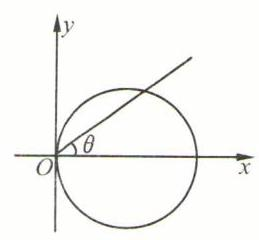
\includegraphics[width=0.2\textwidth]{bodyxb/src/bo_d20aucref24c73anc48g_115_1163_541_259_240_0.jpg}
\end{center}


[第 19(1)题]

19. (1) 如图,以过原点的直线的倾斜角 $\theta$ 为参数,则圆 ${x}^{2} + {y}^{2} - {2x} = 0$ 的参数方程是\blkda{}.

(2)以过点 $A\left( {0,4}\right)$ 的直线的斜率 $t$ 为参数,则椭圆 $4{x}^{2} + {y}^{2} = {16}$ 的参数方程是\blkda{}.

*20. (1) 直线 $\left\{  \begin{array}{l} x = 1 + \dfrac{1}{2}t, \\  y =  - 3\sqrt{3} + \dfrac{\sqrt{3}}{2}t \end{array}\right.$ ( $t$ 为参数)与圆 ${x}^{2} + {y}^{2} = {16}$ 交于 $A,B$ 两点,求 ${AB}$ 中点的坐标.

(2)过点 $P\left( {1,5}\right)$ 的直线 $\left\{  \begin{array}{l} x = 1 + t, \\  y = 5 + \sqrt{3}t \end{array}\right.$ ( $t$ 为参数)与圆 ${x}^{2} + {y}^{2} = {16}$ 交于 $A,B$ 两点,求 $\left| {PA}\right|  + \left| {PB}\right|$ .

(3)过点 $P\left( {1, - 2}\right)$ 作直线,交椭圆 ${x}^{2} + 2{y}^{2} = 8$ 于 $A,B$ 两点,且 $\left| {PA}\right|  \cdot  \left| {PB}\right|  = \dfrac{2}{3}$ ,求此直线的倾斜角.

21. (1) 求直线 $\left\{  \begin{array}{l} x = 2 + \dfrac{t}{2}, \\  y = \dfrac{\sqrt{3}}{2}t \end{array}\right.$ ( $t$ 为参数) 被双曲线 ${x}^{2} - {y}^{2} = 1$ 所截得的弦长.

(2)直线 $l$ 过曲线 $\left\{  \begin{array}{l} x = 2 + 2{t}^{2}, \\  y = 1 - \sqrt{3}t \end{array}\right.$ ( $t$ 为参数)的顶点,且倾斜角为 $\alpha$ ,若 $l$ 被此曲线截得的弦长为 1,求 $\alpha$ .

(3)过抛物线 ${y}^{2} = {4x}$ 的焦点 $F$ 引一条弦 ${AB}$ ,若 $\left| {FA}\right|  : \left| {FB}\right|  = 1 : 2$ ,求直线 ${AB}$ 的方程.

*22. (1) 过点 $M\left( {-2,4}\right)$ 引倾斜角为 $\dfrac{3}{4}\pi$ 的直线交抛物线 ${y}^{2} = {2px}(p >$ 0) 于 $P,Q$ 两点 (如图),若 $\left| {MP}\right| ,\left| {PQ}\right| ,\left| {MQ}\right|$ 依次成等比数列,求 $p$ 的值.

\begin{center}
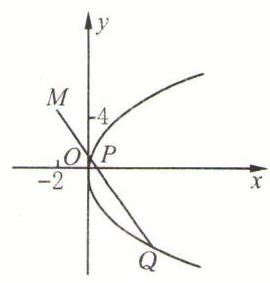
\includegraphics[width=0.2\textwidth]{bodyxb/src/bo_d20aucref24c73anc48g_116_1211_147_270_283_0.jpg}
\end{center}


[第 22(1)题]

(2)已知直线 $y = x + m$ 和曲线 ${x}^{2} + 2{y}^{2} + {4y} - 1 = 0$ 交于 $A,B$ 两点, $P$ 是这条直线上的点,且 $\left| {PA}\right|  \cdot  \left| {PB}\right|  = 2$ ,当 $m$ 变化时,求点 $P$ 的轨迹方程.

23. 已知圆 ${x}^{2} + {y}^{2} = 4$ 上的动点 $B,C$ 始终使 $\angle {BAC} = \dfrac{\pi }{3}$ ,其中 $A\left( {2,0}\right)$ 为定点 (如图).

\begin{center}
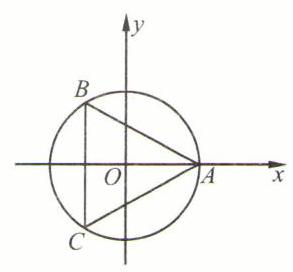
\includegraphics[width=0.2\textwidth]{bodyxb/src/bo_d20aucref24c73anc48g_116_1191_518_293_272_0.jpg}
\end{center}


(第 23 题)

(1)设点 $B$ 在角 $\theta$ 的终边上,其中 $0 < \theta  < \dfrac{4\pi }{3}$ ,写出点 $B$ , $C$ 的坐标.

(2)求 $\bigtriangleup {ABC}$ 重心的轨迹方程.

*24. 已知实数 $x,y$ 满足 $3{x}^{2} + 2{y}^{2} = {6x}$ . 求:

(1) $x + y$ 的最大值.

(2) ${x}^{2} + {y}^{2}$ 的取值范围.

25. (1) 过点 $B\left( {0, - b}\right)$ 作椭圆 $\dfrac{{x}^{2}}{{a}^{2}} + \dfrac{{y}^{2}}{{b}^{2}} = 1\left( {a > b > 0}\right)$ 的弦,求弦长的最大值.

(2)如图,已知椭圆 $\dfrac{{x}^{2}}{{a}^{2}} + \dfrac{{y}^{2}}{{b}^{2}} = 1$ 的长轴为 $A{A}^{\prime }$ ,直线 $l$ 的方程是 $x = \dfrac{{a}^{2}}{c}$ , $P$ 为椭圆上一点, 直线 ${AP},{A}^{\prime }P$ 分别交 $l$ 于点 $M,N$ ,求证: ${FM}\bot {FN}$ .

(3)如图,已知 $A$ 是椭圆长轴的一个端点, $O$ 是椭圆的中心,若椭圆上存在一点 $P$ ,使得 $\angle {OPA} = {90}^{ \circ  }$ ,求椭圆离心率的取值范围.

(4)已知 $P,Q$ 分别是圆 ${x}^{2} + {\left( y - 2\right) }^{2} = 1$ 与双曲线 ${x}^{2} - {y}^{2} = 1$ 上的动点,求 $\left| {PQ}\right|$ 的最小值.

\begin{center}
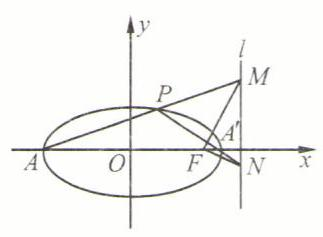
\includegraphics[width=0.2\textwidth]{bodyxb/src/bo_d20aucref24c73anc48g_116_293_1520_323_237_0.jpg}
\end{center}


[第 25(2)题]

\begin{center}
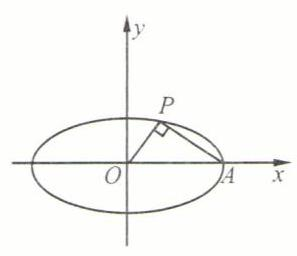
\includegraphics[width=0.2\textwidth]{bodyxb/src/bo_d20aucref24c73anc48g_116_679_1502_297_256_0.jpg}
\end{center}


[第 25(3)题]

\begin{center}
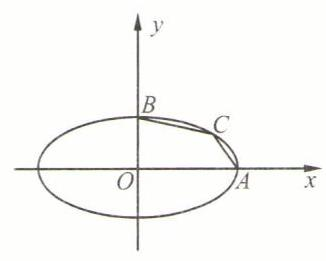
\includegraphics[width=0.2\textwidth]{bodyxb/src/bo_d20aucref24c73anc48g_116_1038_1497_326_261_0.jpg}
\end{center}


[第 26(1)题]

26. (1) 已知 $A,B$ 分别是椭圆 ${x}^{2} + 4{y}^{2} = 4$ 的右顶点与上顶点, $C$ 是椭圆在第一象限弧上的任意一点 (如图),求四边形 ${OACB}$ 面积的最大值 $O$ 为原点).

(2)动线段 ${CD}$ 的一个端点 $C$ 在椭圆 $\dfrac{{x}^{2}}{9} + \dfrac{{y}^{2}}{25} = 1$ 上运动,另一端点在 $x$ 轴上移动. 已知 $\left| {CD}\right|  = 5$ ,利用椭圆的参数方程,求 ${CD}$ 的中点 $M$ 的轨迹方程.

27. 已知长为 1 的线段 ${AB}$ (点 $A$ 在点 $B$ 左侧) 在 $x$ 轴上移动,又 $P\left( {0,1}\right) ,Q\left( {{1.7},2}\right)$ 为两定点 (如图).

(1)设 $A\left( {t,0}\right)$ ,写出直线 ${PA}$ , ${QB}$ 的方程.

(2)求直线 ${PA}$ , ${QB}$ 交点的轨迹方程.

\begin{center}
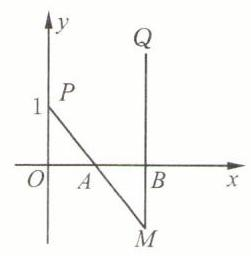
\includegraphics[width=0.2\textwidth]{bodyxb/src/bo_d20aucref24c73anc48g_117_250_371_251_256_0.jpg}
\end{center}


(第 27 题)

\begin{center}
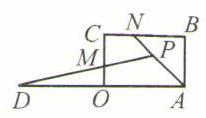
\includegraphics[width=0.2\textwidth]{bodyxb/src/bo_d20aucref24c73anc48g_117_650_496_206_118_0.jpg}
\end{center}


[第 28(1)题]

\begin{center}
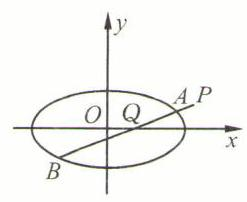
\includegraphics[width=0.2\textwidth]{bodyxb/src/bo_d20aucref24c73anc48g_117_1004_426_247_202_0.jpg}
\end{center}


[第 28(2)题]

28. (1) 已知矩形 ${OABC}$ 的边长 $\left| {OA}\right|  = a,\left| {OC}\right|  = b$ ,点 $D$ 在 ${AO}$ 延长线上, $\left| {OD}\right|  = a$ (如图),设 $M,N$ 分别为边 ${OC},{BC}$ 上的动点,且 $\dfrac{OM}{MC} = \dfrac{BN}{NC} \neq  0$ ,建立适当坐标系,求直线 ${DM}$ 与 ${AN}$ 的交点 $P$ 的轨迹方程.

$* \left( 2\right)$ 已知椭圆 ${x}^{2} + 2{y}^{2} = 8$ 和定点 $P\left( {4,1}\right)$ ,过点 $P$ 作直线交椭圆于 $A,B$ 两点 (点 $A$ 在 $P$ , $B$ 之间),在线段 ${AB}$ 上取点 $Q$ ,使 $\vv{AP} = \lambda \vv{PB},\vv{AQ} =  - \lambda \vv{QB}$ (如图),求动点 $Q$ 的轨迹方程.

*29. 已知抛物线 $y = {x}^{2} - {2x} + 2$ 和过原点、倾斜角为 $\alpha$ 的直线交于 ${P}_{1},{P}_{2}$ 两点,点 $Q$ 在线段 ${P}_{1}{P}_{2}$ 上,且满足 $\dfrac{1}{\left| O{P}_{1}\right| } + \dfrac{1}{\left| O{P}_{2}\right| } = \dfrac{2}{\left| OQ\right| }$ (如图).

(1)写出直线 ${P}_{1}{P}_{2}$ 的参数方程.

(2)把点 $Q$ 的坐标表示成 $\alpha$ 的函数,当 $\alpha$ 在 $\left( {0,\dfrac{\pi }{2}}\right)$ 内变动时,求点 $Q$ 的轨迹的普通方程.

\begin{center}
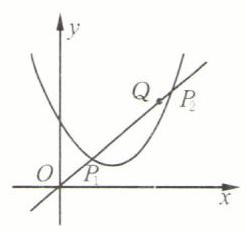
\includegraphics[width=0.2\textwidth]{bodyxb/src/bo_d20aucref24c73anc48g_117_383_1453_246_233_0.jpg}
\end{center}


(第 29 题)

\begin{center}
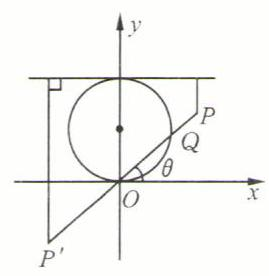
\includegraphics[width=0.2\textwidth]{bodyxb/src/bo_d20aucref24c73anc48g_117_823_1412_269_276_0.jpg}
\end{center}


(第 30 题)

* 30. 过原点的一条直线,交圆 ${x}^{2} + {\left( y - 1\right) }^{2} = 1$ 于点 $Q$ ,在直线 ${OQ}$ 上取一点 $P$ ,使点 $P$ 到直线 $y = 2$ 的距离等于 $\left| {PQ}\right|$ (如图),求当这条直线绕原点旋转时点 $P$ 的轨迹.

\section*{二、极坐标}

\section*{(一) 极坐标的概念}

\section*{【典型题型和解题技巧】}

利用极坐标求动点轨迹.

1. 转移代入法.

例 1 如图 9,点 $A$ 在直线 $x = 5$ 上移动,等腰 $\bigtriangleup {OPA}$ 的顶角 $\angle {OPA}$ 为 ${120}^{ \circ  }$ (点 $O,P,A$ 按顺时针方向排列),求点 $P$ 的轨迹方程.

\begin{center}
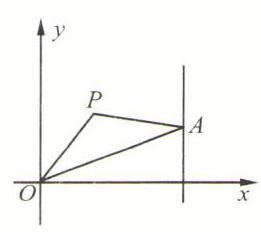
\includegraphics[width=0.2\textwidth]{bodyxb/src/bo_d20aucref24c73anc48g_118_1228_628_261_232_0.jpg}
\end{center}


(图 9)

解 取 $O$ 为极点, $x$ 正半轴为极轴建立极坐标系,则直线 $x = 5$ 的方程为 $\rho \cos \theta  = 5$ .

设点 $P,A$ 坐标依次为 $\left( {\rho ,\theta }\right) ,\left( {{\rho }_{0},{\theta }_{0}}\right)$ ,则 ${\rho }_{0} = \sqrt{3}\rho ,{\theta }_{0} = \theta  - {30}^{ \circ  }$ ,代入 ${\rho }_{0}\cos {\theta }_{0} = 5$ ,得 $\sqrt{3}\rho \cos \left( {\theta  - {30}^{ \circ  }}\right)  = 5$ ,此即为点 $P$ 的轨迹的极坐标方程,展开化成直角坐标方程为 ${3x} + \sqrt{3}y = 0$ .

2. 综合法.

*例 2 过定点 $A\left( {m,0}\right) \left( {m > 0}\right)$ 作直线交 $y$ 轴于 $Q$ 点,过点 $Q$ 作 ${QP} \bot  {AQ}$ 交 $x$ 轴于点 $P$ , 在 ${PQ}$ 的延长线上取点 $M$ ,使 $\left| {MQ}\right|  = \left| {PQ}\right|$ (图 10). 当直线 ${AQ}$ 变动时,求点 $M$ 的轨迹方程.

解 取点 $A$ 为极点, ${Ax}$ 为极轴建立极坐标系.

\begin{center}
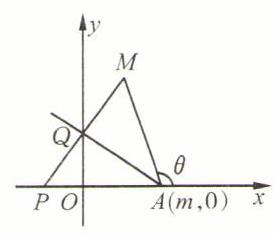
\includegraphics[width=0.2\textwidth]{bodyxb/src/bo_d20aucref24c73anc48g_118_1215_1222_276_234_0.jpg}
\end{center}


(图 10)

设点 $M$ 的坐标为 $\left( {\rho ,\theta }\right)$ ,由已知,易有 $\angle {APQ} = \dfrac{\theta }{2},\left| {AM}\right|  = \left| {AP}\right|$ ,

则 $\left| {AQ}\right|  = \rho \sin \dfrac{\theta }{2},\left| {OA}\right|  = \rho {\sin }^{2}\dfrac{\theta }{2}$ ,

$\therefore \rho  \cdot  \dfrac{1 - \cos \theta }{2} = m$ ,即 $\rho  = \dfrac{2m}{1 - \cos \theta }$ ,化为直角坐标方程为 ${y}^{2} = {4mx} + 4{m}^{2}.$

此即为点 $M$ 的轨迹方程,它是一条抛物线.

\section*{【训练题】}

(A) 31. 在极坐标系中,若等边 $\bigtriangleup {EFG}$ (点 $E,F,G$ 顺时针排列) 的顶点 $E,F$ 分别是 $E\left( {2,\dfrac{\pi }{4}}\right)$ , $F\left( {2,\dfrac{5}{4}\pi }\right)$ ,则顶点 $G$ 的极坐标可能是 (   )

(A) $\left( {4,\dfrac{3}{4}\pi }\right)$ . (B) $\left( {2\sqrt{3},\dfrac{3}{4}\pi }\right)$ . (C) $\left( {2\sqrt{3},\pi }\right)$ . (D) $\left( {3,\pi }\right)$ .

32. 直角坐标为(-3,4)的点的极坐标可能是(   )

(A) $\left( {5,\arctan \left( {-\dfrac{4}{3}}\right) }\right)$ . (B) $\left( {5,\arcsin \dfrac{4}{5}}\right)$ .

(C) $\left( {-5, - \arccos \dfrac{3}{5}}\right)$ . (D) $\left( {-5,\arccos \left( {-\dfrac{3}{5}}\right) }\right)$ .

33. 极坐标方程 $\sin \theta  = \dfrac{1}{3}\left( {\rho  \in  \mathbf{R}}\right)$ 表示的曲线是 (   )

(A) 两条相交直线. (B) 两条射线.

(C) 一条直线. (D) 一条射线.

34. 圆的半径是 1, 圆心的极坐标是 (1,0), 则这个圆的极坐标方程是 (   )

(A) $\rho  = \cos \theta$ . (B) $\rho  = \sin \theta$ . (C) $\rho  = 2\cos \theta$ . (D) $\rho  = 2\sin \theta$ .

35. 极坐标方程 ${3\rho }{\sin }^{2}\dfrac{\theta }{2} = 1$ 表示的曲线是 (   )

(A) 圆. (B) 椭圆. (C) 双曲线. (D) 抛物线.

36. 圆 $\rho  = a\cos \theta  + b\sin \theta$ 与极轴相切的充要条件是(   )

(A) ${ab} = 0$ . (B) ${ab} \neq  0$ . (C) $a = 0,b \neq  0$ . (D) $a \neq  0,b = 0$ .

* 37. 极坐标方程 ${\rho }^{2} - \left( {\theta  + 3}\right) \rho  + {3\theta } = 0$ 表示的曲线是 (   )

(A) 两个圆. (B) 一条直线与一个圆.

(C) 一条直线与一条等速螺线. (D) 一个圆与一条等速螺线.

38. 在极坐标系中,

(1)若 $A\left( {3,\dfrac{\pi }{3}}\right) ,B\left( {-4,\dfrac{7}{6}\pi }\right)$ ,则 $\left| {AB}\right|  =$ \blkda{}, $\bigtriangleup  {AOB}$ 的面积等于\blkda{} $(O$ 为极点).

(2)曲线 $\theta  = 0,\theta  = \dfrac{\pi }{3}\left( {\rho  \geq  0}\right)$ 和 $\rho  = 4$ 所围成的面积是\blkda{}.

(3)已知直线 $\rho \sin \theta  = 3$ 和圆 $\rho  = 3\sin \theta$ ,则圆心到这条直线的距离等于\blkda{}.

(4)圆 $\rho  = 3\cos \theta  + 4\sin \theta$ 的圆心的极坐标是\blkda{},半径是\blkda{}.

(5)根据条件,写出点 $P\left( {2,\dfrac{3\pi }{7}}\right)$ 其他形式的极坐标:

① $\rho  > 0, - {2\pi } < \theta  \leq  0$ ；\blkda{},

② $\rho  < 0,0 \leq  \theta  < {2\pi }$ ；

39. 分别写出下列点、曲线关于极轴、极点、直线 $\theta  = \dfrac{\pi }{2}\left( {\rho  \in  \mathbf{R}}\right)$ 、直线 $\theta  = \dfrac{\pi }{4}\left( {\rho  \in  \mathbf{R}}\right)$ 对称的点的坐标和曲线方程.

(1)点 $\left( {2,\dfrac{\pi }{6}}\right)$ (规定 $\rho  > 0, - \pi  \leq  \theta  < \pi$ ).

(2)曲线 $\rho  = \dfrac{4}{2\cos \theta  + 3\sin \theta }$ .

40. 分别将下列曲线的极坐标方程化成直角坐标方程:

(1) $\rho {\sin }^{2}\dfrac{\theta }{2} = 1$ ；\blkda{} (2) ${\rho }^{2}\cos \theta  - \rho  = 0$ :\blkda{}.

(3) $\sin \theta  = \dfrac{\sqrt{2}}{2}\left( {\rho  > 0}\right)$ :\blkda{}. (4) $\rho  = \cos \theta  + 2\sin \theta$ :\blkda{}.

(5) $\rho  + \dfrac{6}{\cos \theta } = 0$ ；\blkda{}. (6) ${\rho }^{2} = \dfrac{4\left( {{\rho }^{2}{\sin }^{2}\theta  - 1}\right) }{{\cos }^{2}\theta }$ :\blkda{}.

(7) ${\rho }^{2} - {5\rho } - 6 = 0\left( {\rho  \in  \mathbf{R}}\right)$ :\blkda{}.

41. (1) 已知直线 $\rho  = \dfrac{1}{a\cos \theta  + b\sin \theta }$ 与圆 $\rho  = {2c}\cos \theta \left( {c > 0}\right)$ 相切,求证: ${b}^{2}{c}^{2} + {2ac} = 1$ .

(2)已知抛物线 $\rho  = \dfrac{8\cos \theta }{{\sin }^{2}\theta }\left( {\rho  > 0, - \pi  \leq  \theta  < \pi }\right)$ 上的点 $M$ 的极径等于点 $M$ 到准线的距离, 求点 $M$ 的极坐标.

(3)已知两圆的极坐标方程为 $\rho  = 2\cos \theta$ 和 ${\rho }^{2} - 2\sqrt{3}\rho \sin \theta  + 2 = 0$ ,求证:两圆外切,并求切点的极坐标.

\section*{(B)}

42. 在极坐标系中,已知两点 $P\left( {{\rho }_{1},{\theta }_{1}}\right)$ 与 $Q\left( {{\rho }_{2},{\theta }_{2}}\right)$ 满足 ${\rho }_{1} + {\rho }_{2} = 0,{\theta }_{1} + {\theta }_{2} = 0$ ,则 $P,Q$ 两点的位置关系是(   )

(A) 关于极点对称. (B) 关于极轴对称.

(C) 重合. (D) 关于直线 $\theta  = \dfrac{\pi }{2}$ 对称.

43. 已知曲线 $C$ 与曲线 $\rho  = 5\sqrt{3}\cos \theta  - 5\sin \theta$ 关于极轴对称,则曲线 $C$ 的方程是 (   )

(A) $\rho  =  - {10}\cos \left( {\theta  - \dfrac{\pi }{6}}\right)$ . (B) $\rho  = {10}\cos \left( {\theta  - \dfrac{\pi }{6}}\right)$ .

(C) $\rho  =  - {10}\cos \left( {\theta  + \dfrac{\pi }{6}}\right)$ . (D) $\rho  = {10}\cos \left( {\theta  + \dfrac{\pi }{6}}\right)$ .

44. 在极坐标平面上,集合 $P = \left( {\rho ,\theta }\right) \sin \theta  =  - \dfrac{1}{2},\rho  \in  \mathbf{R}$ . 与集合 $S = \left( {\rho ,\theta }\right) \cos \theta  = \dfrac{\sqrt{3}}{2},\rho  \in  \mathbf{R}$ 之间的关系是(   )

(A) $P \subseteq  S$ . (B) $P \supseteq  S$ . (C) $P = S$ . (D) $P \cap  S = \{ \left( {0,0}\right) \}$ .

45. (多选) 圆 ${\rho }^{2} - {2a\rho }\cos \left( {\theta  - \alpha }\right)  + {a}^{2} - {r}^{2} = 0\left( {0 \leq  \alpha  < {2\pi }\text{ 且 }a,r > 0}\right)$ 与极轴相切于极点的条件是(   )

(A) $a = r,\alpha  = 0$ . (B) $a = r,\alpha  = \dfrac{\pi }{2}$ . (C) $a = r,\alpha  = \pi$ . (D) $a = r,\alpha  = \dfrac{3\pi }{2}$ .

* 46.(1)等速螺线共有三圈,曲线始点离开中心为 ${20}\mathrm{{cm}}$ ,最远点离开中心为 ${35}\mathrm{{cm}}$ ,则曲线方程是\blkda{}.

(2)等速螺线过两点 ${P}_{1}\left( {{22},\dfrac{\pi }{6}}\right)$ 与 ${P}_{2}\left( {44.2\pi }\right)$ ,则它的极坐标方程是\blkda{}.

47. 求下列曲线的极坐标方程:

(1) 过点 $\left( {3,\dfrac{\pi }{3}}\right)$ 和 $\left( {3,\dfrac{\pi }{6}}\right)$ 的直线.

(2)以点 $\left( {{\rho }_{0},{\theta }_{0}}\right) \left( {{\rho }_{0} \neq  0,{\theta }_{0} \neq  {k\pi },k \in  \mathbf{Z}}\right)$ 为圆心且过极点的圆.

(3) 以 $\left( {{\rho }_{0},{\theta }_{0}}\right)$ 为圆心, $R$ 为半径的圆.

48. 椭圆 $\dfrac{{x}^{2}}{{a}^{2}} + \dfrac{{y}^{2}}{{b}^{2}} = 1\left( {a > b > 0}\right)$ 上有两点 $A,B$ 满足 ${OA} \bot  {OB}(O$ 为坐标原点)(如图). 求证:

\begin{center}
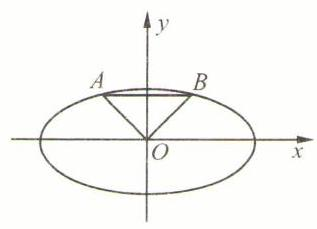
\includegraphics[width=0.2\textwidth]{bodyxb/src/bo_d20aucref24c73anc48g_121_1078_423_317_229_0.jpg}
\end{center}


(第 48 题)

(1) $\dfrac{1}{O{A}^{2}} + \dfrac{1}{O{B}^{2}}$ 为定值.

(2)点 $O$ 到直线 ${AB}$ 的距离为定值.

49. (1)已知 $P$ 是直线 $\rho \sin \theta  = 2$ 上的动点,点 $Q$ 在线段 ${OP}$ 上,且满足 $\left| {OP}\right|  \cdot  \left| {OQ}\right|  = 1$ ,求点 $Q$ 的轨迹方程.

(2)设圆 $C : \rho  = {10}\cos \theta$ 与极轴交于点 $A$ ,由极点 $O$ 引圆 $C$ 的弦 ${OQ}$ ,延长 ${OQ}$ 至点 $P$ ,使 $\left| {QP}\right|  = \left| {AQ}\right|$ ,求动点 $P$ 的轨迹方程.

(3)自原点向圆 ${x}^{2} + {y}^{2} - {2ax} + {a}^{2} - {b}^{2} = 0\left( {a > 0,b > 0}\right)$ 的切线引垂线(如图),求垂足 $P$ 的轨迹的极坐标方程.

\begin{center}
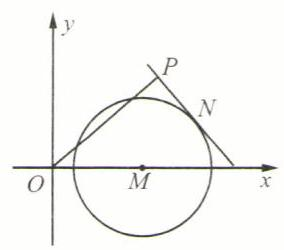
\includegraphics[width=0.2\textwidth]{bodyxb/src/bo_d20aucref24c73anc48g_121_389_1064_284_250_0.jpg}
\end{center}


[第 49(3)题]

\begin{center}
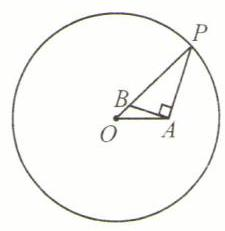
\includegraphics[width=0.2\textwidth]{bodyxb/src/bo_d20aucref24c73anc48g_121_936_1076_225_231_0.jpg}
\end{center}


[第 49(4)题]

(4)已知定圆的圆心是 $O$ ,半径为 $r$ ,圆内有一个定点 $A,\left| {OA}\right|  = a,P$ 是圆上的动点,过点 $A$ 作 ${AB}\bot {AP}$ ,交 ${OP}$ 或其反向延长线于点 $B$ (如图),以圆心 $O$ 为极点,射线 ${OA}$ 为极轴建立坐标系,求点 $B$ 轨迹的极坐标方程.

50. (1) 连接极点 $O$ 和曲线 $\rho  = \dfrac{3}{\cos \theta  - \sin \theta }$ 上的动点 $P$ ,若点 $M$ 满足 $\vv{OM} = \dfrac{m}{n}\vv{MP}$ ,求点 $M$ 的轨迹方程.

(2)已知 $\mathrm{{Rt}}\bigtriangleup {ABO}$ 的直角顶点 $A$ 在直线 $\rho \cos \theta  = 9$ 上移动( $O$ 为原点), $\angle {AOB} = {30}^{ \circ  }$ ,求顶点 $B$ 的轨迹的极坐标方程.

\begin{center}
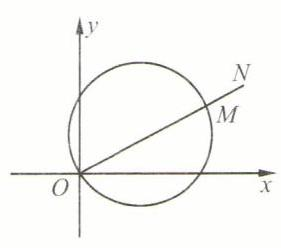
\includegraphics[width=0.2\textwidth]{bodyxb/src/bo_d20aucref24c73anc48g_121_1113_1721_281_248_0.jpg}
\end{center}


[第 50(4)题]

(3) $A$ 是定圆 $B$ 外一定点( $\left| {AB}\right|  = a, \odot  B$ 半径为 $r$ ), $P$ 是 $\odot  B$ 上的动点,以 ${AP}$ 为一边作正三角形 ${APQ}$ (点 $A,P,Q$ 按逆时针方向排列),以 $A$ 为极点,射线 ${AB}$ 为极轴建立极坐标系,求点 $Q$ 的轨迹方程.

(4)已知 $M$ 是圆 ${13}{x}^{2} + {13}{y}^{2} - {15x} - {36y} = 0$ 上的动点, $N$ 在射线 ${OM}$ 上,且满足 $\left| {OM}\right|$

\begin{itemize}
\item $\left| {ON}\right|  = {12}$ (如图),求点 $N$ 的轨迹方程.
\end{itemize}

\section*{*(二) 圆锥曲线的统一极坐标方程}

\section*{【典型题型和解题技巧】}

1. 圆锥曲线统一极坐标方程的应用.

以圆锥曲线的焦点 (椭圆的左焦点、双曲线的右焦点、抛物线的焦点) 为极点,过极点引相应准线的垂线的反向延长线为极轴,则圆锥曲线的统一极坐标方程为 $\rho  = \dfrac{ep}{1 - e\cos \theta }$ . (*

其中 $e$ 为离心率, $p$ 是焦点到相应准线的距离.

圆锥曲线中, 与焦点弦 (过焦点的弦)、焦半径有关的一类问题, 宜利用统一的极坐标方程求解.

例 1 过曲线 $5{x}^{2} - 4{y}^{2} + {10x} + {16y} - {31} = 0$ 的右焦点,引倾斜角为 $\arccos \left( {-\dfrac{\sqrt{3}}{3}}\right)$ 的直线, 交曲线于 $A,B$ 两点,求 $\left| {AB}\right|$ .

解 将原方程化为 $\dfrac{{\left( x + 1\right) }^{2}}{4} - \dfrac{{\left( y - 2\right) }^{2}}{5} = 1$ ,于是 $a = 2,b = \sqrt{5},c = 3$ ,

$\therefore p = \dfrac{{b}^{2}}{c} = \dfrac{5}{3},e = \dfrac{3}{2}$ .

取双曲线的右焦点为极点,双曲线的极坐标方程为 $\rho  = \dfrac{\dfrac{3}{2} \cdot  \dfrac{5}{3}}{1 - \dfrac{3}{2}\cos \theta }$ ,即 $\rho  = \dfrac{5}{2 - 3\cos \theta }$ .

设 $A\left( {{\rho }_{1},\alpha }\right)$ ,则 $B\left( {{\rho }_{2},\pi  + \alpha }\right)$ ,于是

\[
\left| {AB}\right|  = \left| {{\rho }_{1} + {\rho }_{2}}\right|  = 5\left| {\dfrac{1}{2 - 3\cos \alpha } + \dfrac{1}{2 + 3\cos \alpha }}\right|  = \left| \dfrac{20}{4 - 9{\cos }^{2}\alpha }\right|  = \left| \dfrac{20}{4 - 9 \cdot  \dfrac{1}{3}}\right|  = {20}.
\]

注意(1)当 $e > 1$ 时,若限定 $\rho  > 0$ ,则上述统一方程表示双曲线的右支,若允许 $\rho  \in  \mathbf{R}$ ,则上述统一方程也包括双曲线的左支.

(2)过双曲线右焦点的直线,有三种可能:

① 和双曲线右支交于两点,此时焦点弦长为 ${\rho }_{1} + {\rho }_{2}$ ；

②和双曲线只有一个交点,此时直线与渐近线平行；

③和双曲线左、右支各交于一点,此时焦点弦长为 $- \left( {{\rho }_{1} + {\rho }_{2}}\right)$ .

例 2 过抛物线 ${y}^{2} = {2px}$ 的焦点 $F$ 的弦 ${AB}$ 与 $x$ 轴斜交, $M$ 为 ${AB}$ 中点, ${MN} \bot  {AB}$ ,并交 $x$ 轴于点 $N$ (图 11),求证: ${\left| MN\right| }^{2} = \left| {AF}\right|  \cdot  \left| {BF}\right|$ .

\begin{center}
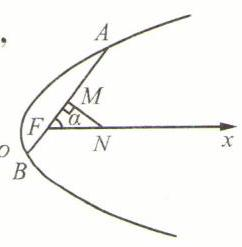
\includegraphics[width=0.2\textwidth]{bodyxb/src/bo_d20aucref24c73anc48g_122_1239_1816_242_247_0.jpg}
\end{center}


(图 11)

证明 取 $F$ 为极点, ${Fx}$ 为极轴建立极坐标系,则抛物线的极坐标方程为 $\rho$  $= \dfrac{p}{1 - \cos \theta }.$

设点 $A,B$ 的坐标依次为 $\left( {{\rho }_{1},\alpha }\right) ,\left( {{\rho }_{2},\pi  + \alpha }\right)$ ,于是

$\left| {AF}\right|  \cdot  \left| {BF}\right|  = \dfrac{p}{1 - \cos \alpha } \cdot  \dfrac{p}{1 + \cos \alpha } = \dfrac{{p}^{2}}{{\sin }^{2}\alpha }.$

不妨设 $0 < \alpha  < \dfrac{\pi }{2}$ ,则 $\left| {MF}\right|  = \dfrac{1}{2}\left( {{\rho }_{1} - {\rho }_{2}}\right)  = \dfrac{p}{2}\left( {\dfrac{1}{1 - \cos \alpha } - \dfrac{1}{1 + \cos \alpha }}\right)  = \dfrac{p\cos \alpha }{{\sin }^{2}\alpha }$ ,

$\therefore \left| {MN}\right|  = \left| {MF}\right|  \cdot  \tan \alpha  = \dfrac{p}{\sin \alpha }$ ,故 ${\left| MN\right| }^{2} = \dfrac{{p}^{2}}{{\sin }^{2}\alpha }$ ,

$\therefore {\left| MN\right| }^{2} = \left| {AF}\right|  \cdot  \left| {BF}\right|$ .

2. 圆锥曲线非统一型极坐标方程的应用.

在直角坐标系中,若取原点为极点, $x$ 正半轴为极轴建立极坐标系,则两坐标系下,圆锥曲线的对应方程分别为

$\dfrac{{x}^{2}}{{a}^{2}} + \dfrac{{y}^{2}}{{b}^{2}} = 1$ 和 $\dfrac{1}{{\rho }^{2}} = \dfrac{{\cos }^{2}\theta }{{a}^{2}} + \dfrac{{\sin }^{2}\theta }{{b}^{2}},$

$\dfrac{{x}^{2}}{{a}^{2}} - \dfrac{{y}^{2}}{{b}^{2}} = 1$ 和 $\dfrac{1}{{\rho }^{2}} = \dfrac{{\cos }^{2}\theta }{{a}^{2}} - \dfrac{{\sin }^{2}\theta }{{b}^{2}},$

${y}^{2} = {2px}$ 和 $\rho  = {2p}\dfrac{\cos \theta }{{\sin }^{2}\theta }.$

由于极点位置的特殊,因此,对于某些和椭圆、双曲线过中心的弦、半径,抛物线过顶点的弦有关的问题, 用以上极坐标方程求解, 常会带来方便.

例 ${3A},B$ 为双曲线 $\dfrac{{x}^{2}}{{a}^{2}} - \dfrac{{y}^{2}}{{b}^{2}} = 1\left( {0 < a < b}\right)$ 上两点,且 ${OA}\bot {OB}$ (图 12),求证: $\dfrac{1}{{\left| OA\right| }^{2}} + \dfrac{1}{{\left| OB\right| }^{2}}$ 为定值.

\begin{center}
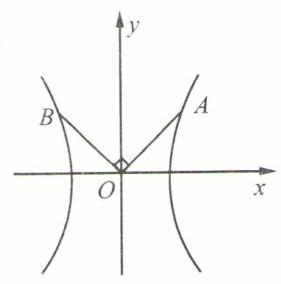
\includegraphics[width=0.2\textwidth]{bodyxb/src/bo_d20aucref24c73anc48g_123_1096_1089_281_284_0.jpg}
\end{center}


(图 12)

证明 取原点 $O$ 为极点, $x$ 正半轴为极轴,建立极坐标系,则双曲线的方程为 $\dfrac{1}{{\rho }^{2}} = \dfrac{{\cos }^{2}\theta }{{a}^{2}} - \dfrac{{\sin }^{2}\theta }{{b}^{2}}$ .

设点 $A$ 的坐标为 $\left( {{\rho }_{1},\alpha }\right)$ ,则点 $B$ 的坐标为 $\left( {{\rho }_{2},\dfrac{\pi }{2} + \alpha }\right)$ . 于是

$\dfrac{1}{{\left| OA\right| }^{2}} + \dfrac{1}{{\left| OB\right| }^{2}} = \left( {\dfrac{{\cos }^{2}\alpha }{{a}^{2}} - \dfrac{{\sin }^{2}\alpha }{{b}^{2}}}\right)  + \left( {\dfrac{{\sin }^{2}\alpha }{{a}^{2}} - \dfrac{{\cos }^{2}\alpha }{{b}^{2}}}\right)  = \dfrac{1}{{a}^{2}} - \dfrac{1}{{b}^{2}}$ (定值).

例 4 过抛物线 ${y}^{2} = {2px}\left( {p > 0}\right)$ 的顶点 $O$ ,作两垂直之弦 ${OA}$ , ${OB}$ (图 13),求 $\bigtriangleup {AOB}$ 面积的最小值.

\begin{center}
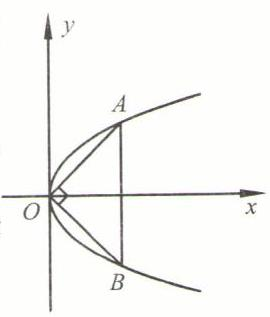
\includegraphics[width=0.2\textwidth]{bodyxb/src/bo_d20aucref24c73anc48g_123_1135_1629_270_317_0.jpg}
\end{center}


(图 13)

解 取原点为极点, $x$ 正半轴为极轴建立极坐标系,则抛物线方程为 $\rho$  $= \dfrac{{2p}\cos \theta }{{\sin }^{2}\theta }$ . 设点 $B$ 的坐标为 $\left( {{\rho }_{1},\alpha }\right)$ ,则点 $A$ 的坐标为 $\left( {{\rho }_{2},\dfrac{\pi }{2} + \alpha }\right)$ ,于是 ${S}_{\bigtriangleup {AOB}} = \dfrac{1}{2}\left| {\dfrac{{2p}\cos \alpha }{{\sin }^{2}\alpha } \cdot  \dfrac{{2p}\cos \left( {\dfrac{\pi }{2} + \alpha }\right) }{{\sin }^{2}\left( {\dfrac{\pi }{2} + \alpha }\right) }}\right|  = \dfrac{2{p}^{2}}{\left| \sin \alpha \cos \alpha \right| } = \dfrac{4{p}^{2}}{\left| \sin 2\alpha \right| } \geq  4{p}^{2}$ ,即 $\bigtriangleup {AOB}$ 面积的最小值为 $4{p}^{2}$ .

\section*{$* \left( \vv{a}\right)$}

51. 设椭圆的极坐标方程是 $\rho  = \dfrac{4}{2 - \lambda \cos \theta }$ ,那么 $\lambda$ 的取值范围是 (   )

(A) $0 < \lambda  < 1$ . (B) $1 < \lambda  < 2$ . (C) $0 < \lambda  < 2$ . (D) $2 < \lambda  < 4$ .

52. 若椭圆的极坐标方程是 $\rho  = \dfrac{5}{3 - 2\cos \theta }$ ,则它的短轴长是(   )

(A) $\dfrac{10}{3}$ . (B) $\sqrt{5}$ . (C) $2\sqrt{5}$ . (D) $2\sqrt{3}$ .

53. 已知圆锥曲线的极坐标方程 $\rho  = \dfrac{5}{3 - 2\cos \theta }$ ,那么它的焦点到相应的准线的距离是(   )

(A) 5 . (B) $\dfrac{5}{2}$ . (C) $\dfrac{5}{3}$ . (D) $\dfrac{2}{3}$ .

54. 在极坐标平面上,过曲线 $\rho  = \dfrac{3}{2 - \cos \theta }$ 的中心,且与极轴垂直的直线方程是 (   )

(A) $\rho  = \cos \theta$ . (B) $\rho  = \cos {2\theta }$ . (C) $\rho \cos \theta  = 1$ . (D) $\rho \cos \theta  = 2$ .

55. 若曲线的极坐标方程为 $\rho  = \dfrac{9}{4 - 5\cos \theta }$ ,则它的焦点的极坐标为 (   )

(A) $\left( {0,0}\right) ,\left( {-9,0}\right)$ . (B) $\left( {0,0}\right) ,\left( {8,0}\right)$ .

(C) $\left( {0,0}\right) ,\left( {8,\pi }\right)$ . (D) $\left( {0,0}\right) ,\left( {{10},\pi }\right)$ .

56. 在极坐标平面上,曲线 $\rho  = \dfrac{1}{1 - 2\cos \theta }$ 的中心坐标是 (   )

(A)(1,0). (B) $\left( {\dfrac{2}{3},0}\right)$ . (C) $\left( {1,\pi }\right)$ . (D) $\left( {\dfrac{2}{3},\pi }\right)$ . $* \left( \vv{b}\right)$ 57. 极坐标方程 $\rho  = \dfrac{k}{{k}^{2} + 1 - {2k}\cos \theta }\left( {k > 0}\right)$ 所表示的曲线是 (   ) (A) 圆. (B) 椭圆或双曲线. (C) 双曲线或抛物线. (D) 椭圆或抛物线. 58. 若极坐标方程 $\rho  = \dfrac{1}{6 - {\mathrm{C}}_{n}^{2}\cos \theta }\left( {n \in  \vv{n}}\right)$ 表示椭圆,则它表示的椭圆的个数是 (   ) (A) 1 . (B) 2. (C) 6. (D) $n$ . 59. 在极坐标系中,椭圆 $\rho  = \dfrac{ep}{1 - e\cos \theta }$ 的长轴是 (   ) (A) $\dfrac{2ep}{1 + {e}^{2}}$ . (B) $\dfrac{ep}{1 - {e}^{2}}$ . (C) $\dfrac{2ep}{1 - {e}^{2}}$ . (D) $\dfrac{1 - {e}^{2}}{2ep}$ .

60. 在极坐标平面上,直线 $\theta  = \dfrac{\pi }{3}\left( {\rho  \in  \mathbf{R}}\right)$ 被圆锥曲线 $\rho  = \dfrac{2}{3 - 2\cos \theta }$ 所截得的弦长等于 (   )

(A) 2 . (B) $\dfrac{3}{2}$ . (C) $\dfrac{7}{5}$ . (D) 1 .

61. 在极坐标平面上,已知 $\rho \cos \theta  =  - 2$ 是曲线 $\rho  = \dfrac{4}{3 - 2\cos \theta }$ 的一条准线,则另一条准线的极坐标方程是(   )

(A) $\rho \cos \theta  = 2$ . (B) $\rho \cos \theta  = \dfrac{18}{5}$ .

(C) $\rho \cos \theta  = 4$ . (D) $\rho \cos \theta  = \dfrac{26}{5}$ .

62. (1) 在极坐标平面上,以极点(0,0)为焦点,以直线 $\rho \cos \theta  =  - 3$ 为准线的抛物线方程是\blkda{}.

(2)已知一椭圆的焦点在极点,两顶点的极坐标为(3,0)和 $\left( {1,\pi }\right)$ ,则椭圆的极坐标方程为\blkda{}.

63. (1)椭圆 $\rho  = \dfrac{8}{3 - \cos \theta }$ 两焦点间的距离等于\blkda{}.

(2)椭圆 $\rho  = \dfrac{9}{5 - 4\cos \theta }$ 的离心率为\blkda{},长轴长是\blkda{},两准线间的距离是\blkda{}.

( 3 )椭圆 $\rho  = \dfrac{3}{3 - 2\cos \theta }$ 中心的极坐标为\blkda{}.

(4)椭圆 $\rho  = \dfrac{6}{2 - \cos \theta }$ 的准线方程为\blkda{}.

(5)椭圆 $\rho  = \dfrac{1}{2 - \cos \theta }$ 的中心到准线的距离是\blkda{}.

(6)椭圆 $\rho  = \dfrac{16}{5 - 3\cos \theta }$ 焦点的极坐标是\blkda{}.

(7)双曲线 $\rho  = \dfrac{2}{1 - 2\cos \theta }$ 的两条渐近线所夹锐角为\blkda{}.

(8)双曲线 $\rho  = \dfrac{1}{3 - 4\cos \theta }\left( {\rho  \in  \mathbf{R}}\right)$ 的实轴长为\blkda{},虚轴长为\blkda{}.

(9)双曲线 $\rho  = \dfrac{ep}{1 - e\cos \theta }\left( {\rho  \in  \mathbf{R}}\right)$ 顶点的极坐标是\blkda{}.

( 10 )抛物线 $\rho  = \dfrac{2}{3 - 3\cos \theta }$ 的焦点到顶点的距离 $=$ \blkda{}.

64. (1) 求过椭圆 $\rho  = \dfrac{2}{3 - \cos \theta }$ 的左焦点,且倾斜角为 $\dfrac{\pi }{4}$ 的弦长.

(2)过曲线 $\rho  = \dfrac{2}{1 - 3\cos \theta }$ 的右焦点作一条倾斜角为 ${60}^{ \circ  }$ 的直线 $l$ ,求 $l$ 被曲线截得的弦长.

(3)已知椭圆 $\rho  = \dfrac{3}{2 - \cos \theta }\left( {0 \leq  \theta  < {2\pi }}\right)$ 的三条焦半径 $\left| {OA}\right| ,\left| {OB}\right| ,\left| {OC}\right|$ 依次成等差数列,且 ${OA},{OC}$ 对应的极角分别为 $\dfrac{\pi }{4}$ 和 $\dfrac{3\pi }{4}$ ,求点 $B$ 的极坐标.

(4)已知椭圆长轴 $\left| {{A}_{1}{A}_{2}}\right|  = 6$ ,焦距 $\left| {{F}_{1}{F}_{2}}\right|  = 4\sqrt{2}$ ,过椭圆左焦点 ${F}_{1}$ 作一条直线,交椭圆于 $M,N$ 两点,设 $\angle {F}_{2}{F}_{1}M = \alpha \left( {0 \leq  \alpha  < \pi }\right)$ ,当 $\alpha$ 取什么值时, $\left| {MN}\right|$ 等于椭圆短轴的长?

(5)过双曲线 $\dfrac{{x}^{2}}{9} - \dfrac{{y}^{2}}{16} = 1$ 的右焦点 $F$ 作倾斜角为 ${45}^{ \circ  }$ 的弦 ${AB}$ (如图),求弦 ${AB}$ 的中点 $C$ 到右焦点 $F$ 的距离.

\begin{center}
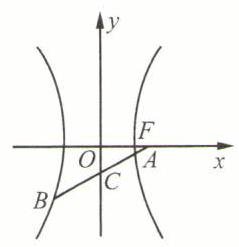
\includegraphics[width=0.2\textwidth]{bodyxb/src/bo_d20aucref24c73anc48g_126_431_682_239_247_0.jpg}
\end{center}


[第 64(5)题]

\begin{center}
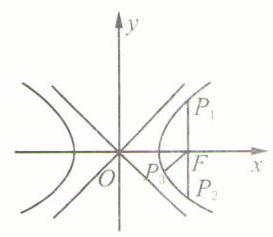
\includegraphics[width=0.2\textwidth]{bodyxb/src/bo_d20aucref24c73anc48g_126_930_688_273_237_0.jpg}
\end{center}


[第 64(6)题]

(6)过双曲线的右焦点 $F$ 作一条垂直于实轴的弦 ${P}_{1}{P}_{2}$ ,过点 $F$ 作一条渐近线的平行线交双曲线于点 ${P}_{3}$ (如图),求证: $\left| {{P}_{1}{P}_{2}}\right|  = 4\left| {{P}_{3}F}\right|$ .

65. 过椭圆的左焦点 $F$ 作长为 8 的弦 ${AB}$ ,已知椭圆的长轴长为 10 ,短轴长为 8 ,求 $\bigtriangleup {AOB}$ 的面积 $(O$ 为椭圆中心).

66. (1) 抛物线 ${y}^{2} = {2px}\left( {p > 0}\right)$ 的一条焦点弦被焦点分成长为 $a,b$ 的两段,求证: $\dfrac{1}{a} + \dfrac{1}{b}$ 为定值.

(2)已知过圆锥曲线焦点的两条弦(若曲线为双曲线,则两弦的 4 个端点在双曲线的同支上) 互相垂直,且其弦长分别为 ${l}_{1},{l}_{2}$ ,求证: $\dfrac{1}{{l}_{1}} + \dfrac{1}{{l}_{2}}$ 为定值.

(C)

67. 动点 $M$ 在 $x$ 轴的正半轴上,过点 $M$ 与定点 $P\left( {2,1}\right)$ 的连线交直线 $y = x\left( {x > 0}\right)$ 于点 $Q$ , 当动点 $M$ 在什么位置时, $\dfrac{1}{\left| PM\right| } + \dfrac{1}{\left| PQ\right| }$ 有最大值?

\begin{center}
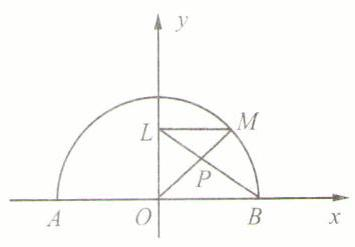
\includegraphics[width=0.3\textwidth]{bodyxb/src/bo_d20aucref24c73anc48g_126_1087_1712_355_247_0.jpg}
\end{center}


(第 68 题)

68. 已知圆的方程为 ${x}^{2} + {y}^{2} = {a}^{2},M$ 为该圆上位于第一象限的点, $L$ 是 $y$ 轴上的点,且 ${ML} \bot  y$ 轴 (如图),求 ${BL}$ 与 ${OM}$ 的交点 $P$ 的轨迹方程.

69. 一条定长为 2 的线段,其两端分别在曲线 ${xy} = 1$ 上移动,求这条线段中点的轨迹方程.

70. 过定点 $A\left( {0,a}\right)$ 的直线 $l$ 与抛物线 $y = {x}^{2}$ 相交于不同的两点 $P,Q$ ,若 $k = \dfrac{1}{\left| AP\right| } + \dfrac{1}{\left| AQ\right| }$ 是不随 $l$ 改变的常数,分别求 $a$ 与 $k$ 的值.

71. 已知直线 $l : \left\{  {\begin{array}{l} x = t\cos \alpha , \\  y = t\sin \alpha  \end{array}\text{ ( }\alpha }\right.$ 为倾角, $t$ 为参数) 和圆 ${\left( x - a\right) }^{2} + {y}^{2} = {r}^{2}\left( {r > 0}\right)$ 交于 $A,B$ 两点,在 $l$ 上求一点 $P$ ,使点 $P$ 满足 $\left| {OA}\right| ,\left| {OP}\right| ,\left| {OB}\right|$ 的倒数依次成等差数列.

72. 已知椭圆 ${\left( x - m\right) }^{2} + 3{\left( y + m\right) }^{2} = 3\left( {m \in  \mathbf{R}}\right)$ .

(1)求证:不论 $m$ 为何实数,这些椭圆的中心总在同一直线 $l$ 上.

(2)平行于 $l$ 的直线中,哪些与椭圆相交？

(3)求证:任一条平行于 $l$ 且与椭圆相交的直线,在每一个椭圆内截得的弦长相等.

73. 当 $m$ 取不同的实数时,方程 $4{x}^{2} + 5{y}^{2} - {8mx} - {20my} + {24}{m}^{2} - {20} = 0$ 表示不同的椭圆,试求一直线,使其被这些椭圆截得的线段长都为 $\dfrac{5}{3}\sqrt{3}$ .

74. 已知 ${PQ}$ 是 $\odot  O$ 的直径 $\left( {{PQ} = {2R}}\right) ,A,B$ 是 ${PQ}$ 上两点, ${MN},{RS}$ 是分别过点 $A,B$ 且与 ${PQ}$ 成 ${45}^{ \circ  }$ 角的两条平行弦 (如图),求证: ${BR} \cdot  {AM} +$  ${BS} \cdot  {AN} \leq  2{R}^{2}$ .

\begin{center}
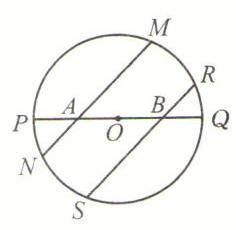
\includegraphics[width=0.2\textwidth]{bodyxb/src/bo_d20aucref24c73anc48g_127_1152_850_236_230_0.jpg}
\end{center}


(第 74 题)

* 75. 过椭圆 $\dfrac{{x}^{2}}{{a}^{2}} + \dfrac{{y}^{2}}{{b}^{2}} = 1$ 的中心 $O$ 依次作 $n\left( {n > 2}\right)$ 条半径 ${r}_{1},{r}_{2},\cdots ,{r}_{n}$ ,每相邻两半径交成 $\dfrac{2\pi }{n}$ 角,求证: $\dfrac{1}{{r}_{1}^{2}} + \dfrac{1}{{r}_{2}^{2}} + \cdots  + \dfrac{1}{{r}_{n}^{2}} = \dfrac{n}{2}\left( {\dfrac{1}{{a}^{2}} + \dfrac{1}{{b}^{2}}}\right)$ .

(注:椭圆的半径是指椭圆上的点与中心的连线段.)

